
\documentclass[a4paper]{article}\usepackage[]{graphicx}\usepackage[]{color}
%% maxwidth is the original width if it is less than linewidth
%% otherwise use linewidth (to make sure the graphics do not exceed the margin)
\makeatletter
\def\maxwidth{ %
  \ifdim\Gin@nat@width>\linewidth
    \linewidth
  \else
    \Gin@nat@width
  \fi
}
\makeatother

\definecolor{fgcolor}{rgb}{0.345, 0.345, 0.345}
\newcommand{\hlnum}[1]{\textcolor[rgb]{0.686,0.059,0.569}{#1}}%
\newcommand{\hlstr}[1]{\textcolor[rgb]{0.192,0.494,0.8}{#1}}%
\newcommand{\hlcom}[1]{\textcolor[rgb]{0.678,0.584,0.686}{\textit{#1}}}%
\newcommand{\hlopt}[1]{\textcolor[rgb]{0,0,0}{#1}}%
\newcommand{\hlstd}[1]{\textcolor[rgb]{0.345,0.345,0.345}{#1}}%
\newcommand{\hlkwa}[1]{\textcolor[rgb]{0.161,0.373,0.58}{\textbf{#1}}}%
\newcommand{\hlkwb}[1]{\textcolor[rgb]{0.69,0.353,0.396}{#1}}%
\newcommand{\hlkwc}[1]{\textcolor[rgb]{0.333,0.667,0.333}{#1}}%
\newcommand{\hlkwd}[1]{\textcolor[rgb]{0.737,0.353,0.396}{\textbf{#1}}}%

\usepackage{framed}
\makeatletter
\newenvironment{kframe}{%
 \def\at@end@of@kframe{}%
 \ifinner\ifhmode%
  \def\at@end@of@kframe{\end{minipage}}%
  \begin{minipage}{\columnwidth}%
 \fi\fi%
 \def\FrameCommand##1{\hskip\@totalleftmargin \hskip-\fboxsep
 \colorbox{shadecolor}{##1}\hskip-\fboxsep
     % There is no \\@totalrightmargin, so:
     \hskip-\linewidth \hskip-\@totalleftmargin \hskip\columnwidth}%
 \MakeFramed {\advance\hsize-\width
   \@totalleftmargin\z@ \linewidth\hsize
   \@setminipage}}%
 {\par\unskip\endMakeFramed%
 \at@end@of@kframe}
\makeatother

\definecolor{shadecolor}{rgb}{.97, .97, .97}
\definecolor{messagecolor}{rgb}{0, 0, 0}
\definecolor{warningcolor}{rgb}{1, 0, 1}
\definecolor{errorcolor}{rgb}{1, 0, 0}
\newenvironment{knitrout}{}{} % an empty environment to be redefined in TeX

\usepackage{alltt}

%--- Load packages. 
\usepackage{amssymb}
\usepackage{amsmath}
\usepackage{framed}

% avoid ugly indentation of paragraphs
\usepackage{parskip}
\usepackage{graphicx}

% open sans font
\usepackage[default,osfigures,scale=0.95]{opensans}

% subfolder with the figures (within manuscript/)
\graphicspath{ {./figures/} }

% for author affiliations
\usepackage{authblk}

%allows inline citations
\usepackage[round]{natbib}
\bibliographystyle{plainnat}

% for degree symbol
\usepackage{gensymb}

% for line numbers
\usepackage{lineno}

% margin size
\usepackage{geometry}
\geometry{verbose,tmargin=3cm,bmargin=3cm,lmargin=3cm,rmargin=3cm}

% for bibtex
% \usepackage{authordate1-4}
% \bibliographystyle{authordate1}

%allows subscripts in text mode
\usepackage{fixltx2e}

%allows rotation of table??
\usepackage{rotating} 

%allows alignment of caption to the left
\usepackage{caption} 
\captionsetup[table]{singlelinecheck=false}

%allows not italic greek letters
\usepackage{textgreek}
\IfFileExists{upquote.sty}{\usepackage{upquote}}{}
\begin{document}


\title{Effects of below-ground space limitation on performance of Eucalyptus seedlings:  Does photosynthesis really control growth?}

\author[1,3]{Courtney E. Campany}
\author[2]{Belinda E. Medlyn}
\author[1]{Remko A. Duursma}

\affil[1]{Hawkesbury Institute for the Environment, University of Western Sydney, Richmond, NSW 2753, Australia}
\affil[2]{Department of Biological Sciences, Macquarie University, North Ryde, NSW 2109, Australia}
\affil[3]{Corresponding author (c.campany@uws.edu.au)}

\renewcommand\Authands{ and }
\maketitle

%--------------------------------------------------------------------------------------------%




%--------------------------------------------------------------------------------------------%

\section*{Abstract}

Intrepreting limitations to plant growth requires understanding of the balance between carbon (\textit{C}) source and sink activity in order to assess carbon allocation and biomass partitioning. This study used manipulations of soil volume to test how growth is coupled to physiology, allocation, and sink activity in Eucalyptus tereticornis seedlings. We grew seedlings in a large range of container sizes and planted containers flush to the soil alongside freely rooted seedlings (free). Reduced soil volume was expected to induce rapid negative effects on growth and physiology compared to free seedlings. It was hypothesized that soil volume effect would be largest in the smallest containers, resulting in physical constraints to growth independently of photosynthesis. Photosynthesis would then become sink-limited, resulting in the build-up of leaf nonstructural carbohydrates eventually leading to photosynthetic down regulation. We observed a negative container effect on aboveground growth soon after the experiment started. Although growth was consistently different across soil volumes mass, partitioning to leaves, stems, roots was conserved after 120 days. Photosynthetic capacity was also significantly reduced in containers, and was related to both leaf nitrogen content and starch accumulation, however starch effects were weaker. We developed a simple seedling growth model that utilized leaf photosynthesis rates to allocate daily \textit{C} uptake towards mass growth of stems, leaves and roots. We then asked whether the observed reductions in photosynthesis explained the observed differences in seedling biomass.  We found that photosynthesis reductions alone were not sufficient and the inclusion of additional carbon and mass allocation strategies were necessary to better predict the observed growth responses to decreasing soil volume. Overall, we found limited evidence for sink-limitation of photosynthesis by constraining seedling growth in containers, and argue that shifts in \textit{C} allocation are necessary to explain the experimental results. This research highlights the need to further understand adaptive strategies of plant \textit{C} allocation, and confirms that photosynthesis and growth are not always directly related.

\section*{Key Words}

photosynthesis, sink regulation, growth, carbon allocation, soil volume


\section*{Introduction}

For plants to grow they need to assimilate sufficient carbon (\textit{C}) to allow the buildup of structural biomass and to fuel the metabolism associated with biomass maintenance \citep{sala2012carbon}.  Roots uptake the nutrients, such as nitrogen (\textit{N}), required for leaf growth and leaves fix the \textit{C} required for growth and maintenance of the entire plant. This growth is driven by several simultaneous processes, including photosynthesis (A), \textit{C} investment among organs, resources acquisition and metabolic costs \citep{korner2006plant, fourcaud2008plant}. Additionally a major component of dry matter investment is a storage pool of carbohydrates used to fuel growth and metabolism when photosynthesis does not meet demand \citep{chapin1990ecology}. The concentration of storage carbohydrates within plant tissues depends on the passive balance between \textit{C} supply, via A, and \textit{C} demands through growth and respiration \citep{mitchell2013drought}, or as an actively regulated process to maintain hydraulic transport across tissues \citep{sala2012carbon}. Thus, understanding plant growth across spatial and temporal scales requires integration of the uptake of \textit{C} and \textit{N} in coalescence, as well as patterns of allocation across plant tissues 

The distribution of assimilated \textit{C} is a primary determinant of plant growth \citep{friedlingstein1999toward}, yet our knowledge of the mechanisms by which allocation is regulated is poor \citep{poorter2012biomass}. The allocation of \textit{C} involves the shifting of the products of A between respiration and biomass production, ephemeral and long-lived tissues, and above and belowground components \citep{litton2007carbon}. With non-limiting availability of nutrients, light, and water a plant should allocate resources to leaves in order to maximize \textit{C} acquisition and height growth.  For balanced growth between leaves and roots it is generally assumed that biomass is preferentially allocated to obtain the most limiting resource, however, it is unlikely that plants ever reach a dynamic equilibrium with allocation as supply rates of light and soil resources fluctuate continuously \citep{shipley2002balanced}. Alternatively, acclimation of plant traits, via phenotypic plasticity of leaf and root morphology, can improve the capacity of resource capture without resulting shifts in biomass allocation \citep{waisel1996plant}, especially in young plants \citep{reich2002root}.  As a result, empirical evidence is needed to understand the mechanisms driving patterns of \textit{C} investment, biomass allocation, and trait acclimation when resource availability is not optimal.

As a consequence of the multitude of mechanisms driving both \textit{A} and \textit{C} allocation there exists ongoing controversy over the hierarchy processes controing plant growth.  Generally, greater rates of \textit{A} are assumed to to produce more growth but this common view both ignores the rules of stoichiometry and neglects processes such as C transport, respiration and storage \citep{korner2013growth}. Futhermore, focus on \textit{C} allocation and storage is often first placed on the fate of carbon that has been recently assimilated by \textit{A} \citep{atkin2015new}. As a result, the inhibition of \textit{A} by sink limitation related to water and nutrient availability or a reduction in whole plant carbon demand with build of non-structural carbohydrates may be incorrectly ignored. As \textit{A} is linked to whole plant physiology by reciprocal controls, these top down views can ignore how source-sink interactions can override direct control of photosynthesis by light and CO\textsubscript{2} \citep{paul2001sink}. When testing how environmental controls affect plant growth it is therefore essential to understand how sink strength of component tissues is affected in combination with \textit{A} in order to understand how \textit{C} allocated within the whole plant.

Plants undergo many physiological and morphological changes in response to rooting volume, potentially affecting root/shoot growth, biomass partitioning, net photosynthetic rate, water relations, nutrient uptake and respiration \citep[and references therein]{nesmith1998effect}. Thus exposing plants differntial soil volumes, via container size, can be used to manipulate seedling growth and subsequently test the mechanisms that affect the balance between \textit{C} sink and source activity.
Recently,a meta-analysis of the effects on rooting volume reported that reduction in growth is mainly caused by a reduction in \textit{A} per unit leaf area \citep{poorter2012pot}, yet the causality of this reduction is unclear. The volume of containers in which plants are grown is thought to decrease the sink strength for \textit{C} by reducing root growth, and plants grown in small containers are more likely to exhibit photosynthetic down-regulation \citep{arp1991effects, mcconnaughay1991physical,gunderson1994photosynthetic, sage1994acclimation, maina2002intra,ronchi2006growth}. Smaller containers may also reduce \textit{N} uptake, either from physical root restriction or decreased supply, and N deficiencies can affect growth, Rubisco limitation, sugar metabolism, and carbohydrate partitioning between source and sink tissues \citep{stitt1991rising, hermans2006plants}. Alternatively, plants in small soil volumes may alter root morphology under root restriction \citep{krizek1985comparative} or leaf morpholgy if nitrogen uptake is altered \citep{reich1998photosynthesis}. By utilizing what is known about the biological constraints of small containers we can empirically test how growth strategies are adapted when seedlings reach differential thresholds of soil volume to exploit. 

This study tests how \textit{Eucalyptus tereticornis} seedlings adjust biomass allocation and physiology across a range of limiting soil volumes and compares these responses to field grown seedlings without root restriction. Seedlings were maintained under well watered conditions and the plasticity of seedlings to maintain optimal photosynthetic capacity and the duration of this response was concomitantly tracked with patterns of biomass allocation and leaf traits to understand processes that regulate seedling growth. Reduced soil volume was expected to induce rapid negative effects on growth and physiology compared to free seedlings. It was hypothesized that soil volume effect would be largest in the smallest containers, resulting in physical constraints to growth independently of photosynthesis. Photosynthesis would then become sink-limited, resulting in the build-up of leaf nonstructural carbohydrates leading to photosynthetic down regulation through time as a function on available soil volume. 

\section*{Methods}

\subsection*{\textit{Experimental Design}}

This experiment was located on the Hawkesbury Forest Experiment site in Richmond, NSW, Australia. Plots were located in open cover with a site history that consists of a paddock that was converted from native pasture grasses. Top soils at this site, used for the study, are an alluvial formation of low-fertility sandy loam soils (380 and 108~mg~kg\textsuperscript{-1} total nitrogen and phosphorus respectively) with low organic matter (0.7~\%) and low water holding capacity. At this site a soil hard layer exists at $\sim$1.0~m with a transition to heavy clay soils. The climate for the region is classified as sub-humid temperate. 

\textit{Eucalyptus tereticornis} seedlings, 20~weeks old and approximately 40~cm tall in tube stock, were chosen from a single local Cumberland plain cohort. Previous experiments have confirmed that species with tap roots (similar to \textit{E. tereticornis}) use the center of the container as the medium for thick roots leaving the periphery of the soil as the most active sites for fine root proliferation \citep{biran1980a,biran1980b}. This is generally hypothesized to be a different response than seedlings with no taproot. By using a species with tap root growth and manipulations of container length rather than width, it is believed that a more realistic test of inhibition of growth through constrained soil volume would be achieved. Six seedlings were harvested before planting to measure initial leaf area and dry mass of leaves, stems and roots.

Six container volumes were used ranging from 5~l to 3~l, with a 22.5~cm diameter, and lengths ranging from 15 to 100~cm. Containers were constructed of PVC pipe and were filled with local top soil (described above). Soil in each container was packed to achieve a target soil bulk density of 1.7~g~m\textsuperscript{-3}. A Imidacloprid (BAYER CropScience) insecticide tablet was planted 5 cm below the roots for each seedling. Containers were planted flush with the soil surface inside metal sleeves, designed to minimize excess air space between the container and outside soil while also allowing for container removal. This allowed for soil temperatures in containers to reflect conditions of naturally sown seedlings. Each experimental block (n=7) contained a complete replicate set of container volumes as well as one free seedling, with 1 m\textsuperscript{2} spacing. For each free seedling, a 1~m\textsuperscript{2} subplot was excavated to 0.5~m and replaced with the same soil used in each container. Around each subplot a border of root exclusion material was buried 0.25~m deep and extended 0.25~m above the ground surface to exclude local vegetation.

Plants were watered bi-weekly or when needed, accounting for natural precipitation, to maintain soil moisture at field capacity (13-15~\%). To achieve field capacity all soil filled containers were weighed and soil moisture was measured (Time Domain Reflectometer at 10~cm depth) before watering. Derived equations based on container weight at planting (when soil moisture was 3~\%) and at field capacity was used to calculate watering requirements for each individual plant. Drain systems were built into each pot to prevent pooling of water in containers before root expansion, from reduced root uptake, or from large rainfall events. These conditions could lead to an anaerobic environment around the root that could hinder the uptake of water through reduced root conductance \citep{poorter2009causes}, an undesired experimental artifact. A collection compartment in the bottom of containers, containing gravel covered by root exclusion mesh, was used collect water for 20, 25, and 35~l containers. Plastic tubing (6~mm diameter) was inset into the gravel layer and extended through the top of the container. A lysimeter pump was then used to suction excess water, through the tubing, as needed. As small containers (5, 10, and 15~l) have a larger irradiation effect a simple bottom plug was used to drain water from the gravel compartment.  

\subsection*{\textit{Growth and morphology metrics}}
Seedlings were planted on January 21\textsuperscript{st} 2013 and stem height, diameter at 15~cm and leaf count were measured weekly thereafter. Once the growth rate of individual plants had significantly declined a full biomass harvest was completed (May 5\textsuperscript{th} 2013). Dry mass of leaves, stems, roots and cumulative leaf area (LI-3100C Area Meter; LI-COR, Lincoln, NE, USA) was measured for each seedling. Mean individual leaf area for each harvested seedling was calculated by dividing cumulative leaf area by total leaf count of only fully expanded leaves. This value was then used to interpolate cumulative leaf area through time with weekly leaf counts. Root mass was collected by passing soil from each container through a 1~mm sieve, washing, separating into fine and coarse roots (\textless2~mm and \textgreater2~mm diameter, respectively) and then drying to a constant mass. Roots from the free seedlings were collected by excavating each 1~m\textsuperscript{2} subplot to 0.5~m depth.  25~g fresh weight subsamples of washed fine roots were analyzed, using WhinoRhizo software (Regent Instruments Inc.), for specific root length (SRL, cm~m\textsuperscript{-1}).

\subsection*{\textit{Photosynthetic parameters}}
Leaf gas exchange measurements were performed bi-weekly at saturating light (\textit{A}\textsubscript{sat}) and saturating light and [CO\textsubscript{2}] (\textit{A}\textsubscript{max}) on new fully expanded leaves. Measurements were initiated only after new leaf growth occurred (March 17\textsuperscript{th}, 2013), approximately 6 weeks following planting, and continued until the biomass harvest. Leaf level gas exchange was measured with a standard leaf chamber equipped with blue-red light emitting diodes using a portable gas exchange system (LI-6400, LI-COR, Lincoln, NE, USA). \textit{A}\textsubscript{sat} measurements were made at PPFD of 1800~{\textmugreek}mol~m\textsuperscript{-1}~s\textsuperscript{-1} and [CO\textsubscript{2}] of 400~{\textmugreek}l~l\textsuperscript{-1} and \textit{A}\textsubscript{max} with [CO\textsubscript{2}] of 1600~{\textmugreek}l~l\textsuperscript{-1} and PPFD of 1800~{\textmugreek}mol~photons~m\textsuperscript{-1}~s\textsuperscript{-1}. This choice of light level to achieve light saturation is consistent with other studies on \textit{Eucalyptus} species \citep{kallarackal1997ecophysiological,pinkard1998photosynthetic,crous2013photosynthesis,drake2014capacity}. These measurements were conducted during midday (10:00-14:00~h) with leaf temperature maintained at 25$\degree$C. After leaves acclimated to the chamber environment, net CO\textsubscript{2} assimilation rate and stomatal conductance (\textit{g}\textsubscript{s}) were logged 5 times for both \textit{A}\textsubscript{sat} and \textit{A}\textsubscript{max}. Photosynthetic CO\textsubscript{2} response (AC\textsubscript{i}) curves were also devloped at 25$\degree$C on a random subset of each container size (n=3) after new leaves were first produced and immediately prior to the final harvest (May 23\textsuperscript{rd} 2013). Each AC\textsubscript{i} curve began at the reference [CO\textsubscript{2}] of 400~{\textmugreek}l~l\textsuperscript{-1} and then consisted of 12 additional steps from [CO\textsubscript{2}] of 50 to 1800~{\textmugreek}l~l\textsuperscript{-1}at 25$\degree$C and saturating light (above). From these curves the photosynthetic parameters, \textit{J}\textsubscript{max} and \textit{Vc}\textsubscript{max}, can be quantified using biochemical model of \citet{farquhar1980biochemical}. Leaf dark respiration rates (\textit{R}\textsubscript{d}) was measured on each seedling during the same dates as AC\textsubscript{i} curves using detached leaves inside a conifer chamber attached to the Licor 6400 at least 1 hour after sundown.   Measurements were taken at a reference [CO\textsubscript{2}] of 400~{\textmugreek}l~l\textsuperscript{-1} while leaf temperature was maintained at current ambient conditions. Specific leaf area (SLA, m\textsuperscript{2}~kg\textsuperscript{-1}) was calculated by measuring leaf area and dry mass for individual leaves sampled during gas exchange campaigns.

\subsection*{\textit{Leaf water potential}}
Predawn ($\Psi\textsubscript{pd}$) and midday ($\Psi\textsubscript{l}$) leaf water potentials were measured for each seedling using a PMS 1505D pressure chamber (PMS Instruments, Albany, OR, USA) on fully expanded leaves during the same time period as AC\textsubscript{i} and \textit{R}\textsubscript{d}. Leaves were collected, immediately stored inside foil covered bags and then transported to the laboratory for measurements of water potential. $\Psi\textsubscript{pd}$ was measured before sunrise and $\Psi\textsubscript{l}$ at midday 13:00-14:30~h. These measurements were used as a measure of static water stress on the seedlings \citep{sellin1999does}, and to ensure that the bulk soil water availability was high enough for plants as they became larger and roots filled the soil volume. 

\subsection*{\textit{Leaf, root and soil chemistry}}
Leaves used in each gas exchange measurements and subsamples of harvested roots were dried to a constant mass and milled for analysis of \textit{N} content. Pre-planting soil samples (n=6) and subsamples of soil from each container following harvest were sieved to remove organic material, air dried and milled for analysis. \textit{N} concentrations of milled samples were determined using a Carlo Erba CE1110 elemental analyzer with thermal conductivity and mass spectromic detection (of \textit{N}\textsubscript{2} and CO\textsubscript{2}).  The percentage of \textit{N} in the sample was calculated by comparison with known standards. Leaf total non-structural carbohydrates concentration was analyzed using a total starch assay kit (Megazyme International 303 Ireland Ltd., Wicklow, Ireland) on gas exchange leaves (above) and represents the sum of starch (mg~g\textsuperscript{-1}) and soluble sugar (mg~g\textsuperscript{-1}) concentrations. Starch was quantified using a thermostable $\alpha$-amylase and amyloglucosidase assay \citep{McCleary_starch} and soluble sugars were determined following the anthrone method \citep{ebell1969variation}. Full methods of the TNC assay are described in \citep{mitchell2013drought}.

\subsection*{\textit{Seedling growth model}}
We developed a simple seedling growth model that utilized leaf photosynthesis to allocate daily carbon assimilate towards mass production of stems, leaves and roots. The model begins with the mean initial component mass (leaf\textsubscript{i}, stem\textsubscript{i} and root\textsubscript{i}) and a starting leaf area (LA\textsubscript{i}) measured prior to planting. Biomass production for each day of the experiment was estimated by multiplying the whole tree seedling carbon uptake gain per day (\textit{C}\textsubscript{day}) by a carbon use efficiency parameter (\textUpsilon\textsubscript{c}, \citet{makela1997carbon}), allocating new carbon to the previous day’s biomass and then accounting for carbon loss via tissue respiration. \textit{C}\textsubscript{day} was calculated for each seedling by fitting a coupled photosynthesis - stomatal conductance model \citep{farquhar1980biochemical,medlyn2011reconciling} in the 'plantecophys' package in R \citep{Duursma2014} to the mean photosynthetic parameters (R\textsubscript{d}, J\textsubscript{max}, V\textsubscript{cmax}, and g\textsubscript{1}) for each treatment and meteorological data from an onsite weather station.  Examples of the photosynthesis model are described in \citet{medlyn2002temperature} and the approach of the coupled leaf gas exchange model are described in \citet{duursma2014peaked}. The g\textsubscript{1} parameter was generated by fitting observed stomatal conductance values into the optimal stomatal conductance model from \citep{medlyn2012reconciling}. Combined with the meteorological parameters PPFD, air temperature, and relative humidity, at 15~m intervals, photosynthesis rates ({\textmugreek}mol~CO\textsubscript{2}~m\textsuperscript{-2}~s\textsuperscript{-1}) were then predicted for each soil volume treatment. Rates were assumed to be representative of the entire 15~min meteorological interval. \textit{C}\textsubscript{day} was then calculated by converting predicted rates to mass \textit{C} gain over 15~min (g~m\textsuperscript{-2}) and then summed for 24~h. Additionally, it is necessary to calculate a self-shading parameter (\textit{M}) when scaling flat leaf photosynthesis to seedling cumulative leaf area. This was accomplished by utilizing 61 previously digitized Eucalyptus seedlings, covering 5 total species which include \textit{E. tereticornis}, from \citet{duursma2012light} to run in 'YplantQMC' package in R \citep{YplantQMC} to build a 3d plant structure based on digitized metrics of plant allometry and crown structure. Inputting the same physiological parameters listed above, 'YplantQMC' outputs total photosynthesis, using total leaf area, for seedlings assuming self-shading as well as for a full sun large horizontal leaf.  The ratio of self-shading to flat leaf total photosynthesis was then used to calculate \textit{M}, which was then applied to modeled rates of photosynthesis when scaling to seedling cumulative leaf area. All default parameters used in model simulations are reported in Table.~\ref{table:Table3}.

We then utilized this model to to investigate whether the effects of soil volume on photosynthesis were enough to accurately predict overall seedling production after 120 days or whether changes in \textit{C} allocation or mass partitioning where also necessary to predict biomass. First, the model was simulated using only changes in photosynthesis rates across treatments combined with mean values of mass partitioning and either published or local data of stem and root respiration rates. Next, different mass partitioning and \textit{C} allocation scenarios were simulated to investigate sources of missing \textit{C} from the initial model simulation. This included testing model sensitivity by altering leaf \textit{C} allocation, root respiration rates, and fine root \textit{C} allocation. For all cases, mass production was compared between model output and harvested seedlings to investigate what \textit{C} allocation strategies beyond reduction in photosynthesis aid in  prediction of seedling growth responses induced by limiting soil volume. 

\subsection*{\textit{Data Analysis}}
Differences in experimental parameters with soil volume were analysed by one-way analysis of variance (ANOVA) in R with individual containers as random effects and soil volume as a categorical fixed effect. Tukey’s post-hoc tests were performed in conjunction with ANOVA to determine which specific paired comparisons among soil volumes were different. Mixed model ANOVAs of \textit{A}\textsubscript{max} and leaf chemistry were performed using the 'nlme' package \citep{nlme} in R and \textit{r}\textsuperscript{2} values of mixed models were computed as in \citet{nakagawa2013general}. Tests of allometric relationships between biomass components were implemented using major axis regression in the 'smatr' package \citep{warton2012smatr}. Results were considered significant at P$\leq$0.05.

\section*{Results}

\subsection*{\textit{Growth and morphology metrics}}
In this open field study, colder temperatures and reductions in cumulative PPFD per day (Fig.~\ref{fig:figure1}) most likely lead to the reduced growth in the free seedlings in the final weeks of the experiment (Fig.~\ref{fig:figure2}).  Combined with severe growth reductions in the smallest container volumes the experiment was chosen to be harvested after 120~days. Over the 120~days height, diameter, and leaf area diverged between container volumes (Fig.~\ref{fig:figure2}).  First, seedling leaf area significantly diverged between soil volumes (\textit{P}\textless0.026) during the 5\textsuperscript{th} week of the experiment. Following this period both height (8\textsuperscript{th} week) and then diameter (9\textsuperscript{th} week) significantly deviated across soil volumes (\textit{P}\textless0.002 \& 0.001, respectively).  Negative growth effects then manifested as severely reduced height gain and declining leaf area through time with small container volumes across the final two months of the experiment. Seedlings maintained diameter growth throughout the experiment, although marginal with smaller soil volumes in the final month. Final seedling height significantly increased with increasing soil volume (\textit{P}\textless0.001).  Increases in both final stem diameter (\textit{P}\textless0.001) and cumulative leaf area (both \textit{P}\textless0.001) were found with increasing soil volume and these differences were driven mainly by the largest container and the free seedling.

Total plant biomass at harvest was significantly different across container volumes (\textit{P}\textless0.001) and with free seedlings (\textit{P}\textless0.001, Table.~\ref{table:Table1}). We analyzed the relationship between biomass growth with each fold increase in soil volume and found an increase of 34~\% with a doubling of pot size, consistent with the meta-analysis of \citet{poorter2012pot}. Additionally, plant biomass was highly correlated with total leaf area across all treatments (\textit{r}\textsuperscript{2} = .97, \textit{P}\textless0.001). Differences in biomass partitioning to leaves, stems, and roots were not different across soil volumes when variation in seedling biomass within treatments was factored in the analysis. Across all treatments, the final harvested root:shoot was conserved in these seedlings, with a slightly higher shoot than root mass on average ($\overline{x}$=0.904).

SRL of harvested fine roots was not different across soil volumes (Table.~\ref{table:Table1}). Over the duration of the experiment SLA was higher in free seedlings but was not different across containers sizes (Table.~\ref{table:Table1}, \textit{P}\textless0.001) and this pattern was evident in the first gas exchange measurement campaign (6th week, \textit{P}\textless0.001).

\subsection*{\textit{Leaf and root chemistry}}
Leaf \textit{N}~\% was significantly higher in free seedlings and the largest container volume at the onset of gas exchange measurements (6th week, \textit{P}\textless0.001).  Over the remaining duration of the experiment the smallest container volume had a significant reduction in leaf \textit{N}~\% compared to other soil volumes, while the free seedling maintained a greater leaf \textit{N}~\% (Table.~\ref{table:Table1}, \textit{P}\textless0.001).  Additionally, mean leaf starch content in the smallest container was double that of free seedlings (\textit{P}=0.042), while leaf soluble sugars did not differ across treatments throughout the experiment (Table.~\ref{table:Table1}).  Differences in leaf starch between the free seedling and the smallest container were also evident during the first gas exchange campaign (\textit{P}=0.0013). 

\subsection*{\textit{Gas exchange and photosynthetic parameters}}
\textit{A}\textsubscript{sat} (Fig.~\ref{fig:figure3}) and \textit{A}\textsubscript{max} (Table.~\ref{table:Table2}) were both significantly higher in the largest container volume and the free seedling at the first measurement campaign (both \textit{P}\textless0.001). Across measurement campaigns \textit{A}\textsubscript{sat} was consistently higher in free seedlings than in containers (Figure 3, \textit{P}\textless0.001). The interaction between photosynthetic capacity on a mass basis, leaf starch, and foliar \textit{N} was marginally significant (\textit{P}=0.0584) but \textit{A}\textsubscript{max} was highly correlated to both leaf \textit{N} content and leaf starch (both \textit{P}\textless0.001). Across all measurement campaign \textit{A}\textsubscript{max} was higher when foliar \textit{N} was also higher, usually associated with low levels of leaf starch (Fig.~\ref{fig:figure3}a). \textit{A}\textsubscript{max} was also lower when leaf starch was high as higher leaf \textit{N} often did not coincide with high leaf starch (Fig.~\ref{fig:figure3}b)

The photosynthetic parameters \textit{J}\textsubscript{max} and \textit{Vc}\textsubscript{max} were not different across measurement campaigns, therefore the parameter means per volume are reported here (Table.~\ref{table:Table2}).  Overall, both \textit{J}\textsubscript{max} and \textit{Vc}\textsubscript{max} were significantly higher in free seedlings with little variation between container volumes (\textit{P}=0.0012 \& 0.0021, respectively). Leaf dark respiration rates were not significantly different across soil volumes (Table.~\ref{table:Table2}). The \textit{g}\textsubscript{1} parameter, generated for each seedling from the \citet{medlyn2012reconciling} optimal stomatal conductance model, was not different across soil volumes (Table.~\ref{table:Table2}). Predicted values of \textit{g}\textsubscript{s}, using the \textit{g}\textsubscript{1} parameter, where highly correlated with observed values (\textit{r}\textsuperscript{2}= .74, \textit{P}\textless0.001, data not shown).

Neither $\Psi\textsubscript{pd}$ nor $\Psi\textsubscript{l}$ were different across treatments, with mean values of -0.27 and -1.2~mPa across all seedlings, respectively. Although stomatal conductance in free seedlings was generally higher than those in containers (Table.~\ref{table:Table2}, \textit{P}=0.0023), the mean rates for all seedlings were high at 0.37~mol~H\textsubscript{2}0~m\textsubscript{-2}~s\textsubscript{-1} and did not decline significantly across the experiment duration. Combined these indices provide strong evidence that water stress was not apparent on these well-watered seedlings throughout the experiment. Soil \textit{N}~\% at harvest was not different across soil volumes ($\bar{x}$=04.5~\%) and decreased approximately 3~\% across all containers over the experiment duration. This indicates that nutrient leaching from free seedlings or from draining of containers following natural rainfall events did not differ between treatments. 

\subsection*{\textit{Modelling seedling biomass}}
The initial model simulation, testing only treatment specific photosynthesis rates, was unable to accurately predict the responses of actual harvested seedling biomass to reduced soil volume.  When both \textit{C}\textsubscript{day} and biomass of modeled and harvested seedlings were scaled to to the free seedling the initial model design overestimated biomass for all treatments (Fig.~\ref{fig:figure6}a).  This suggests that reductions in photosynthesis alone could not realistically capture the reduced growth response of these seedlings.  Next, the model was re-run using the mean mass fractions of leaves, stems and roots from the final harvest, per treatment, to drive daily mass partitioning and seedling production.  Combined with treatment specific photosynthesis rates this model still overestimated seedling production for all treatments (Fig.~\ref{fig:figure6}b).  

To test whether potential sources of missing \textit{C} could improve the modeled response of seedling mass production the model was run with 3 different \textit{C} allocation scenarios that could not be tested within the framework of this experiment. This was accomplished by testing the sensitivity of the model to adjustments of \textit{C} allocation to leaves or fine roots or root respiration rates by $\pm$50~\% of default values. The model output of these scenarios was then compared to both the original model output and with harvested seedling biomass.  Increasing \textit{C} allocation to either leaves or fine roots,in coalescence with photosynthesis rates, did improve the model but neither were sufficient to accurately predict the actual biomass response  (Fig.~\ref{fig:figureSI1}a,c). Altering respiration rates of fine and coarse roots did not have a noticeable deviation from the original model (Fig.~\ref{fig:figureSI1}b).

\section*{Discussion}


%--------------------------------------------------------------------------------------------%
\section*{Tables}
% Load xtable for printing tables.



%seedling data table
% latex table generated in R 3.1.2 by xtable 1.7-4 package
% Tue Jan 06 17:01:51 2015
\begin{sidewaystable}[ht]
\centering
\caption{Responses of plant and leaf characterisitcs of \textit{Eucalyptus tereticornis} seedlings to soil volume treatments. Each value reflects the mean(standard error) of each treatment.} 
\label{table:Table1}
\begin{tabular}{llllllll}
  \hline
Volume (L) & Seedling~mass~(g) & SLA~(m\textsuperscript{2}~kg\textsuperscript{-1}) & Leaf~Nitrogen~(\%) & Leaf~Sugars~(\%) & Leaf~Starch~(\%) & SRL~(cm~m\textsuperscript{-1}) & Root~Nitrogen~(\%) \\ 
  \hline
5 & 14.8 (1.82) & 9.5 (0.23) & 1.1 (0.02) & 6.4 (0.28) & 12.7 (0.97) & 39.1 (5.47) & 0.82 (0.05) \\ 
  10 & 20.0 (2.38) & 9.8 (0.24) & 1.3 (0.04) & 6.7 (0.25) & 9.4 (0.75) & 34.2 (5.83) & 0.75 (0.02) \\ 
  15 & 25.4 (2.49) & 11.0 (0.47) & 1.4 (0.06) & 7.2 (0.28) & 7.3 (0.73) & 37.6 (4.63) & 0.71 (0.02) \\ 
  20 & 23.4 (1.63) & 9.8 (0.28) & 1.4 (0.05) & 6.6 (0.26) & 9.5 (0.88) & 45.3 (5.50) & 0.76 (0.04) \\ 
  25 & 30.4 (5.49) & 10.4 (0.37) & 1.3 (0.06) & 6.9 (0.24) & 9.8 (0.71) & 47.0 (7.10) & 0.74 (0.02) \\ 
  35 & 52.2 (9.55) & 11.3 (0.44) & 1.5 (0.08) & 6.8 (0.22) & 9.8 (0.65) & 50.6 (11.61) & 0.77 (0.03) \\ 
  Free & 174.5 (18.02) & 13.0 (0.44) & 2.4 (0.09) & 7.4 (0.25) & 6.8 (0.65) & 43.7 (6.24) & 0.87 (0.04) \\ 
   \hline
\end{tabular}
\end{sidewaystable}



%data.df$taxa <- paste("\\emph{",taxa,"}", sep="")

% latex table generated in R 3.1.2 by xtable 1.7-4 package
% Tue Jan 06 17:01:51 2015
\begin{sidewaystable}[ht]
\centering
\caption{Responses of leaf level gas exchange parameters of \textit{Eucalyptus tereticornis} seedlings to soil volume treatments. Each value reflects the mean(standard error) of each treatment. Units for \textit{A}\textsubscript{max} and \textit{R}\textsubscript{dark} are {\textmugreek}mol~m\textsuperscript{-1}~s\textsuperscript{-1} and \textit{g}\textsubscript{s} are mol~m\textsuperscript{-1}~s\textsuperscript{-1}.} 
\label{table:Table2}
\begin{tabular}{lllllll}
  \hline
Volume~(L) & \textit{A}\textsubscript{max} & \textit{R}\textsubscript{dark} & \textit{J}\textsubscript{max} & \textit{Vc}\textsubscript{max} & \textit{g}\textsubscript{s} & \textit{g}\textsubscript{1} \\ 
  \hline
5 & 21.2 (0.9) & 2.8 (0.3) & 103.7 (5.8) & 62.9 (2.8) & 0.30 (0.01) & 5.1 (0.1) \\ 
  10 & 22.3 (1.4) & 2.7 (0.4) & 116.5 (5.9) & 69.4 (2.9) & 0.36 (0.01) & 5.4 (0.1) \\ 
  15 & 23.3 (1.2) & 1.4 (0.1) & 123.1 (15.4) & 79.4 (10.0) & 0.45 (0.01) & 6.2 (0.2) \\ 
  20 & 26.1 (0.7) & 1.7 (0.1) & 130.0 (14.1) & 81.4 (6.0) & 0.38 (0.01) & 5.2 (0.2) \\ 
  25 & 23.9 (0.9) & 1.2 (0.1) & 131.9 (5.9) & 78.6 (2.6) & 0.32 (0.01) & 4.8 (0.2) \\ 
  35 & 25.0 (1.0) & 1.5 (0.2) & 121.2 (3.7) & 78.0 (3.5) & 0.33 (0.02) & 4.7 (0.2) \\ 
  Free & 33.1 (0.7) & 1.3 (0.1) & 171.7 (18.6) & 101.2 (5.7) & 0.49 (0.02) & 5.0 (0.2) \\ 
   \hline
\end{tabular}
\end{sidewaystable}




%--------------------------------------------------------------------------------------------%
\clearpage
\section*{Figures}

%air variables figure
\begin{figure}[h!]
    \centering
    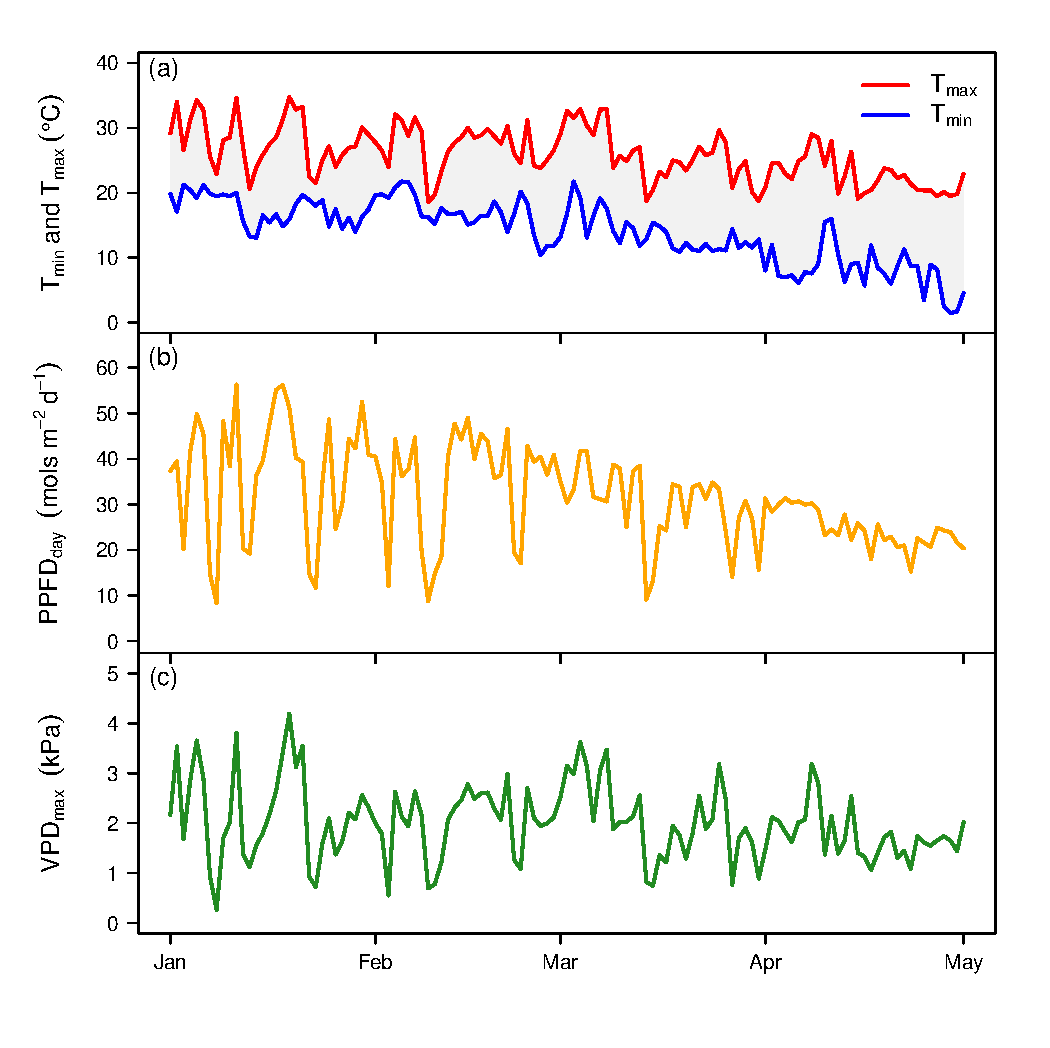
\includegraphics[width=0.99\textwidth]{airvars.pdf}
    \caption{Daily maximum and minimum temperature (a), cumulative daily PPFD (b), and daily maximum vapour pressure deficit (c) across the experiment duration.}
    \label{fig:figure1}
\end{figure}

%allometry figure
\begin{figure}[h!]
    \centering
    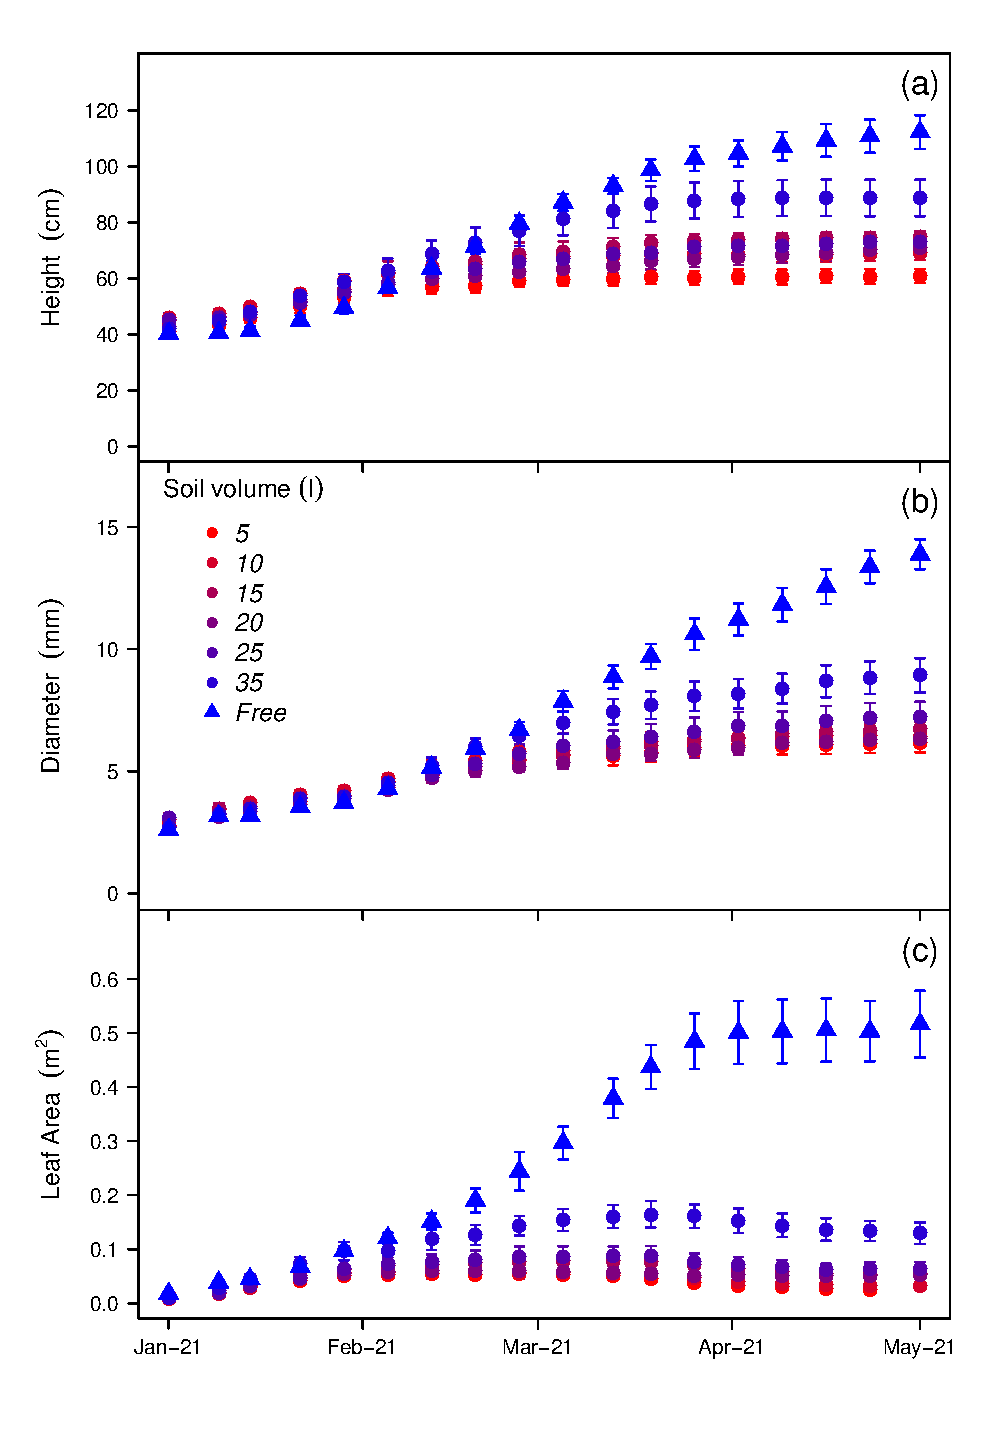
\includegraphics[width=0.99\textwidth]{allometry.pdf}
    \caption{Soil volume treatment means~$\pm$~SE~(n=7) of height growth (a), diameter growth (b), and interpolated seedling leaf area (c) measured weekly of \textit{Eucalyptus tereticornis} seedlings over 120~days.}
    \label{fig:figure2}
\end{figure}

%asat figure
\begin{figure}[h!]
    \centering
    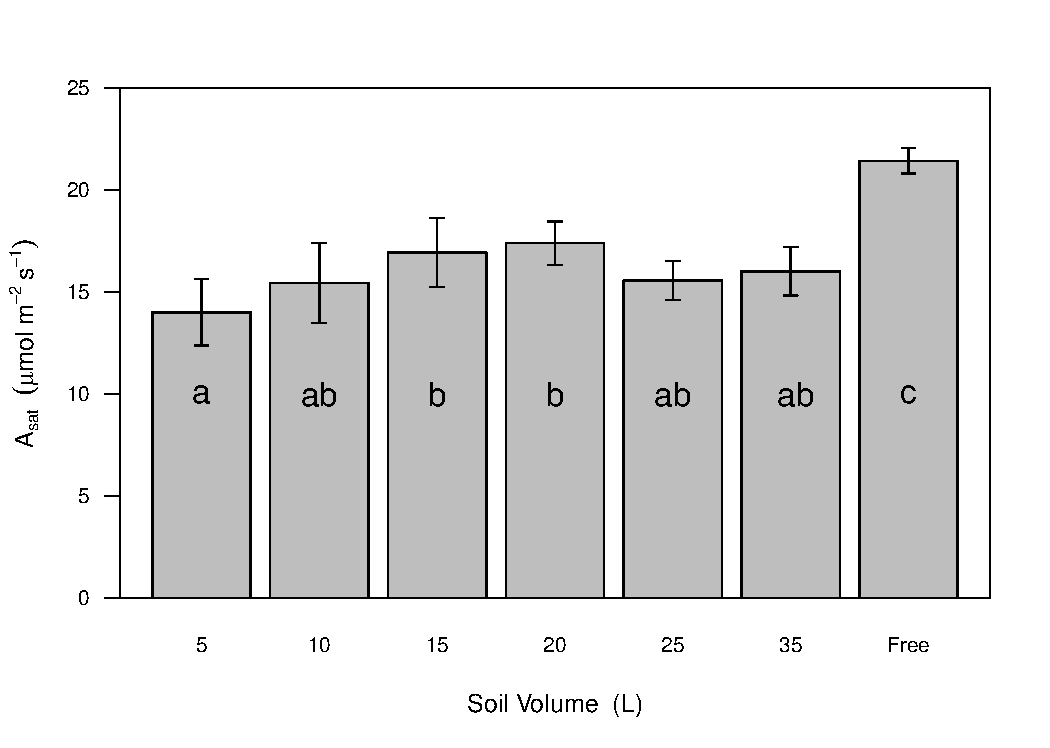
\includegraphics[width=0.99\textwidth]{Asat.pdf}
    \caption{Soil volume treatment means~$\pm$~SE~(n=7), across all measurement dates (n=6), of light saturated rates of photosynthesis at 25$\degree$C}. Different letters represent significant differences between treatments.
    \label{fig:figure3}
\end{figure}

%partitioning figure
\begin{figure}[h!]
    \centering
    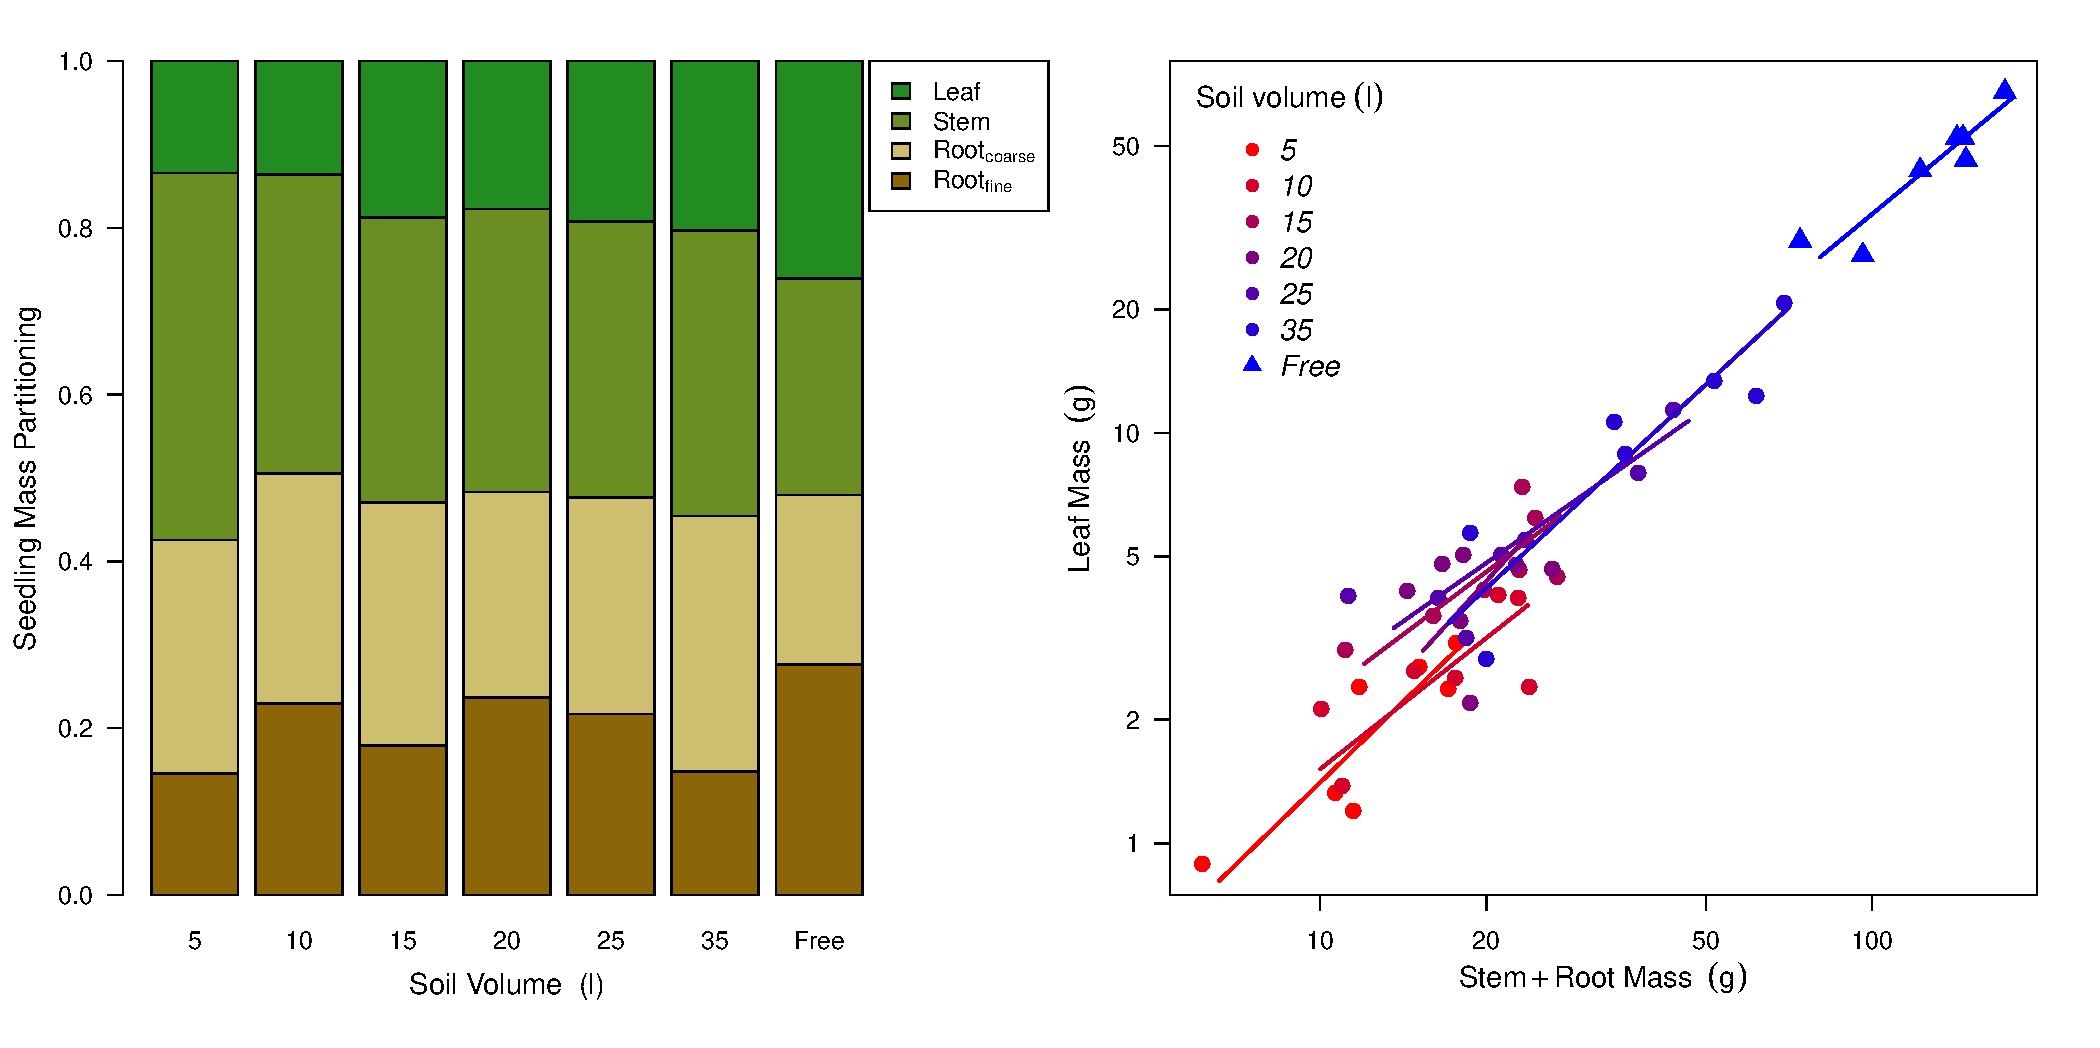
\includegraphics[width=0.99\textwidth]{massfractions.pdf}
    \caption{Soil volume treatment means (n=7) of mass partitioning to leaves, stems, and roots (a) and bi-variate relationships between mass allocation to leaves and stems + roots (b). Lines represent standardized major axis fitting of the log transformed allometric relationships of leaf mass fraction by treatment.}
    \label{fig:figure4}
\end{figure}

%photochem figure
\begin{figure}[h!]
    \centering
    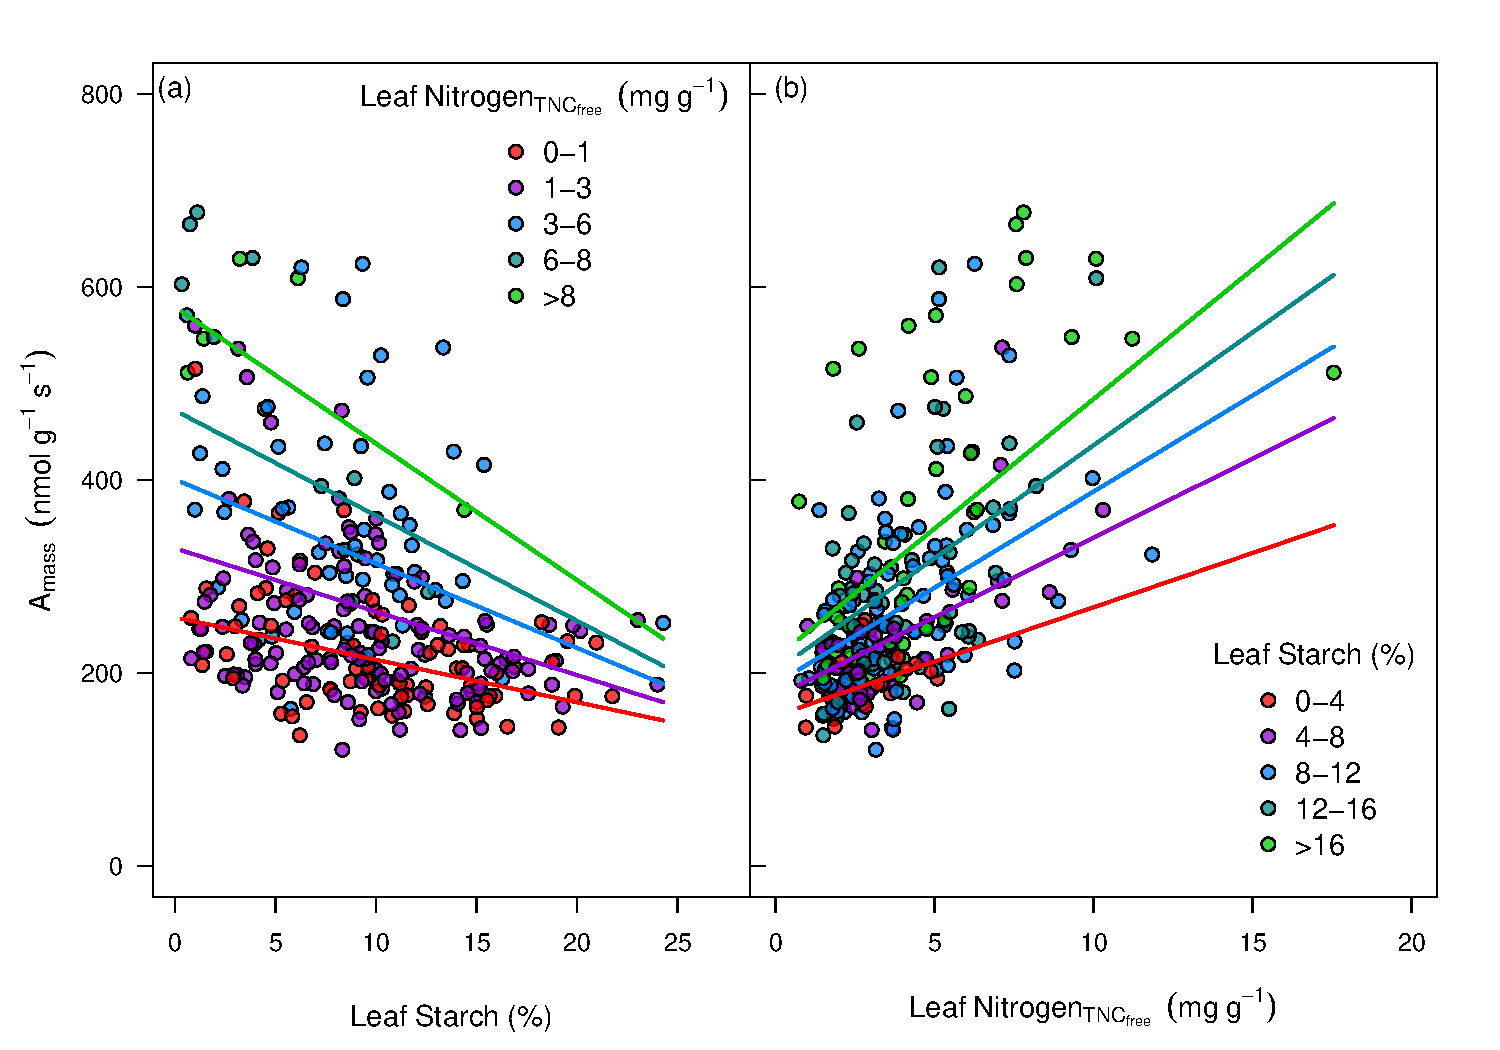
\includegraphics[width=0.99\textwidth]{A_leafchem.pdf}
    \caption{Photosynthetic capacity, on a leaf mass basis, as a function of accumulation of leaf starch (a) and leaf nitrogen content without TNC (b).  Colors represent bins levels (n=5) of both leaf starch and nitrogen grouped from low to high .  Lines represents predictions, for each bin level, from the linear mixed effects model equation of \textit{A}\textsubscript{max} as a function of starch and nitrogen. The marginal \textit{r}\textsuperscript{2} (fixed effects only) was 0.37 and the conditional \textit{r}\textsuperscript{2} (fixed and random effects) was 0.48 for the complete model.}
    \label{fig:figure5}
\end{figure}

%model base figure
\begin{figure}[h!]
    \centering
    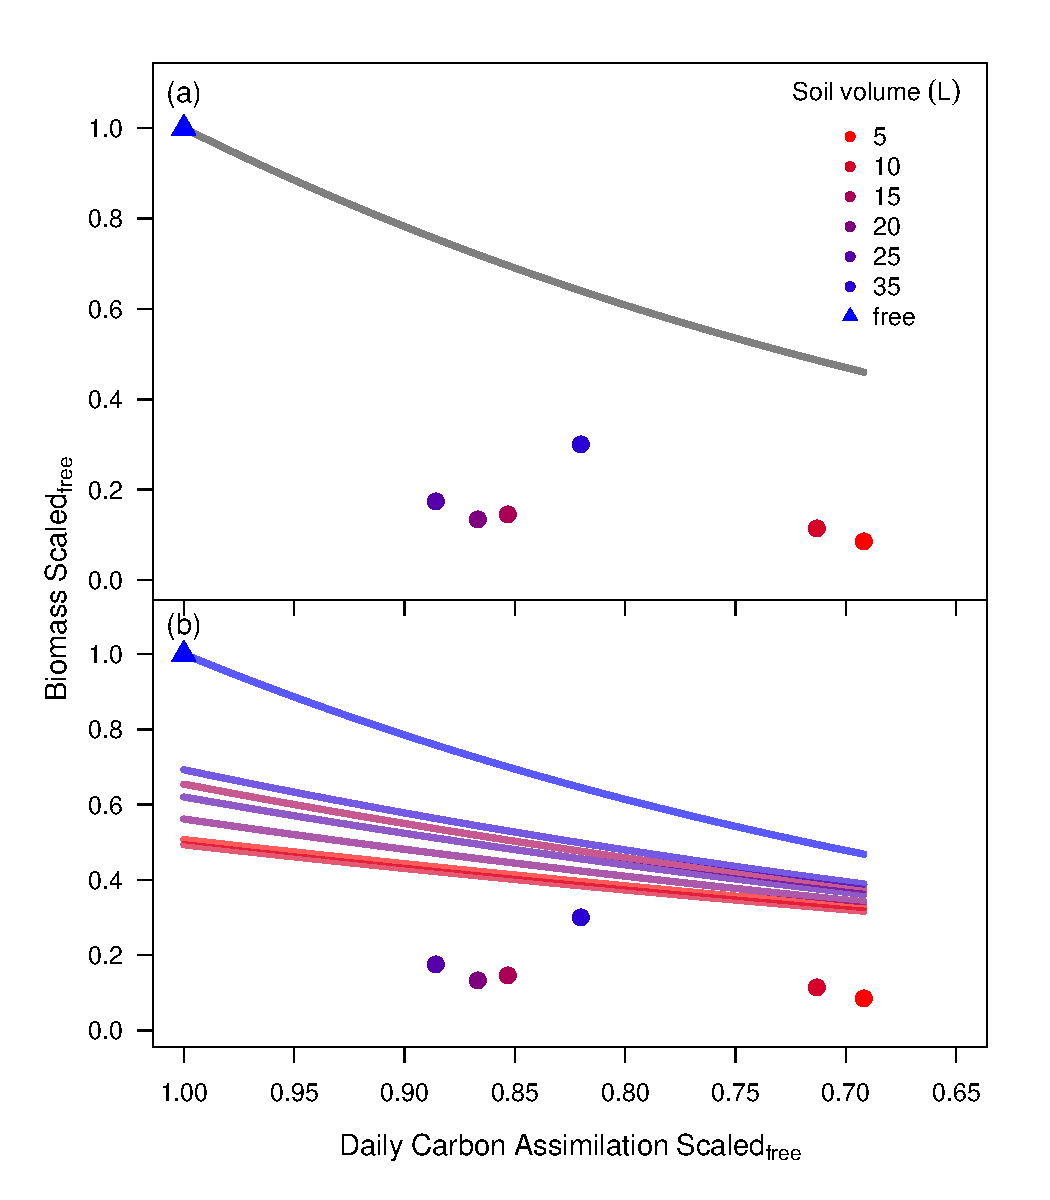
\includegraphics[width=0.99\textwidth]{gC_day.pdf}
    \caption{Modeled and harvested seedling biomass (g) versus daily assimilated carbon gain (g~m\textsuperscript{2}).  Values of biomass and carbon gain are scaled to the free seedling with unlimited soil volume.}
    \label{fig:figure6}
\end{figure}

%--------------------------------------------------------------------------------------------%
\clearpage
\section{Supporting Information Figures}
% Supporting information. Make sure Figures continue with Fig S1 etc.

\renewcommand\thefigure{S\arabic{figure}}    
\setcounter{figure}{0}   


\begin{figure}[h!]
    \centering
    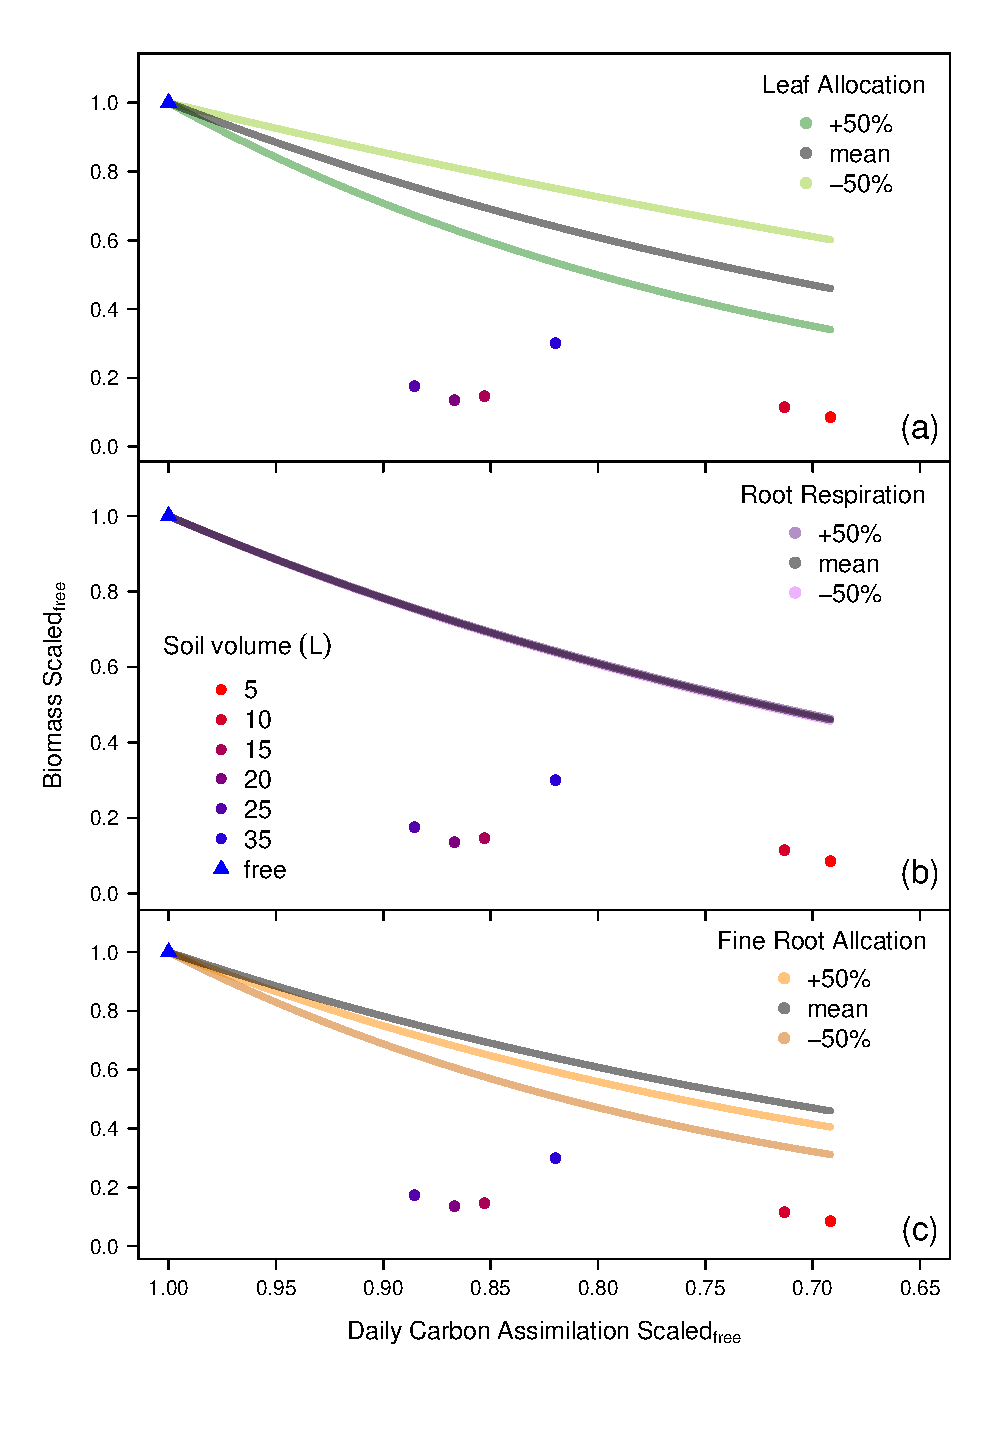
\includegraphics[width=0.99\textwidth]{gc_Day_scenario.pdf}
    \caption{Modeled and harvested seedling biomass (g) versus daily assimilated carbon gain (g~m\textsuperscript{2}) including sensitivity testing for unmeasured carbon allocation scenarios.  Model parameters of leaf allocation (a), root respiration (b), and fine root allocation (c) were increased or decreased by 50$\%$.}
    \label{fig:figureSI1}
\end{figure}


\begin{table}[h!]
  \caption{Seedling Growth Model Default Parameters} 
  \centering 
  \begin{tabular}{l l l l} 
  \hline
  Variable & Default Value & Units & Source  \\ [0.5ex] 
  \hline
  Leaf area\textsubscript{i} & 0.035 & m\textsuperscript{2} & this study \\ 
  Leaf mass\textsubscript{i} & 3.45 & g & this study \\ 
  Stem mass\textsubscript{i} & 1.51 & g & this study \\ 
  Root mass\textsubscript{i} & 0.99 & g & this study \\ 
  \textUpsilon\textsubscript{c} & .65 & g~C g~mass & \citet{makela1997carbon} \\ 
  R\textsubscript{coarse root} & 0.00124 & g~C g~root\textsuperscript{-1} & \citet{marsden2008relating} \\ 
  R\textsubscript{fine root} & 0.010368 & g~C g~root\textsuperscript{-1} & \citet{ryan2010factors} \\ 
  R\textsubscript{stem} & 0.00187 & g~C g~stem\textsuperscript{-1} & Drake 2014 (unpublished) \\ 
  C\textsubscript{day} & 4.7-6.8 & g~C m\textsuperscript{2} & this study \\ 
  M & 0.80-0.87 &  & this study \\ 
  
  \hline 
  \end{tabular}
  \label{table:Table3} 
\end{table}

%--------------------------------------------------------------------------------------------%
\clearpage
\bibliography{pve_cites}

%--------------------------------------------------------------------------------------------%
\end{document}



